% GNUPLOT: LaTeX picture with Postscript
\begingroup
  \makeatletter
  \providecommand\color[2][]{%
    \GenericError{(gnuplot) \space\space\space\@spaces}{%
      Package color not loaded in conjunction with
      terminal option `colourtext'%
    }{See the gnuplot documentation for explanation.%
    }{Either use 'blacktext' in gnuplot or load the package
      color.sty in LaTeX.}%
    \renewcommand\color[2][]{}%
  }%
  \providecommand\includegraphics[2][]{%
    \GenericError{(gnuplot) \space\space\space\@spaces}{%
      Package graphicx or graphics not loaded%
    }{See the gnuplot documentation for explanation.%
    }{The gnuplot epslatex terminal needs graphicx.sty or graphics.sty.}%
    \renewcommand\includegraphics[2][]{}%
  }%
  \providecommand\rotatebox[2]{#2}%
  \@ifundefined{ifGPcolor}{%
    \newif\ifGPcolor
    \GPcolortrue
  }{}%
  \@ifundefined{ifGPblacktext}{%
    \newif\ifGPblacktext
    \GPblacktexttrue
  }{}%
  % define a \g@addto@macro without @ in the name:
  \let\gplgaddtomacro\g@addto@macro
  % define empty templates for all commands taking text:
  \gdef\gplbacktext{}%
  \gdef\gplfronttext{}%
  \makeatother
  \ifGPblacktext
    % no textcolor at all
    \def\colorrgb#1{}%
    \def\colorgray#1{}%
  \else
    % gray or color?
    \ifGPcolor
      \def\colorrgb#1{\color[rgb]{#1}}%
      \def\colorgray#1{\color[gray]{#1}}%
      \expandafter\def\csname LTw\endcsname{\color{white}}%
      \expandafter\def\csname LTb\endcsname{\color{black}}%
      \expandafter\def\csname LTa\endcsname{\color{black}}%
      \expandafter\def\csname LT0\endcsname{\color[rgb]{1,0,0}}%
      \expandafter\def\csname LT1\endcsname{\color[rgb]{0,1,0}}%
      \expandafter\def\csname LT2\endcsname{\color[rgb]{0,0,1}}%
      \expandafter\def\csname LT3\endcsname{\color[rgb]{1,0,1}}%
      \expandafter\def\csname LT4\endcsname{\color[rgb]{0,1,1}}%
      \expandafter\def\csname LT5\endcsname{\color[rgb]{1,1,0}}%
      \expandafter\def\csname LT6\endcsname{\color[rgb]{0,0,0}}%
      \expandafter\def\csname LT7\endcsname{\color[rgb]{1,0.3,0}}%
      \expandafter\def\csname LT8\endcsname{\color[rgb]{0.5,0.5,0.5}}%
    \else
      % gray
      \def\colorrgb#1{\color{black}}%
      \def\colorgray#1{\color[gray]{#1}}%
      \expandafter\def\csname LTw\endcsname{\color{white}}%
      \expandafter\def\csname LTb\endcsname{\color{black}}%
      \expandafter\def\csname LTa\endcsname{\color{black}}%
      \expandafter\def\csname LT0\endcsname{\color{black}}%
      \expandafter\def\csname LT1\endcsname{\color{black}}%
      \expandafter\def\csname LT2\endcsname{\color{black}}%
      \expandafter\def\csname LT3\endcsname{\color{black}}%
      \expandafter\def\csname LT4\endcsname{\color{black}}%
      \expandafter\def\csname LT5\endcsname{\color{black}}%
      \expandafter\def\csname LT6\endcsname{\color{black}}%
      \expandafter\def\csname LT7\endcsname{\color{black}}%
      \expandafter\def\csname LT8\endcsname{\color{black}}%
    \fi
  \fi
    \setlength{\unitlength}{0.0500bp}%
    \ifx\gptboxheight\undefined%
      \newlength{\gptboxheight}%
      \newlength{\gptboxwidth}%
      \newsavebox{\gptboxtext}%
    \fi%
    \setlength{\fboxrule}{0.5pt}%
    \setlength{\fboxsep}{1pt}%
\begin{picture}(8620.00,12940.00)%
      \csname LTb\endcsname%%
      \put(4310,12736){\makebox(0,0){\strut{}Absolute error - Mass, Energy, $\delta \in \{0.05, 0.5\}$}}%
    \gplgaddtomacro\gplbacktext{%
      \colorrgb{0.50,0.50,0.50}%%
      \put(56,10624){\makebox(0,0)[r]{\strut{}10^{-14}}}%
      \colorrgb{0.50,0.50,0.50}%%
      \put(56,10915){\makebox(0,0)[r]{\strut{}10^{-12}}}%
      \colorrgb{0.50,0.50,0.50}%%
      \put(56,11205){\makebox(0,0)[r]{\strut{}10^{-10}}}%
      \colorrgb{0.50,0.50,0.50}%%
      \put(56,11496){\makebox(0,0)[r]{\strut{}10^{-8}}}%
      \colorrgb{0.50,0.50,0.50}%%
      \put(56,11786){\makebox(0,0)[r]{\strut{}10^{-6}}}%
      \colorrgb{0.50,0.50,0.50}%%
      \put(56,12076){\makebox(0,0)[r]{\strut{}10^{-4}}}%
      \colorrgb{0.50,0.50,0.50}%%
      \put(56,12367){\makebox(0,0)[r]{\strut{}10^{-2}}}%
      \colorrgb{0.50,0.50,0.50}%%
      \put(168,10275){\makebox(0,0){\strut{} }}%
      \colorrgb{0.50,0.50,0.50}%%
      \put(582,10275){\makebox(0,0){\strut{} }}%
      \colorrgb{0.50,0.50,0.50}%%
      \put(996,10275){\makebox(0,0){\strut{} }}%
      \colorrgb{0.50,0.50,0.50}%%
      \put(1410,10275){\makebox(0,0){\strut{} }}%
      \colorrgb{0.50,0.50,0.50}%%
      \put(1824,10275){\makebox(0,0){\strut{} }}%
      \colorrgb{0.50,0.50,0.50}%%
      \put(2239,10275){\makebox(0,0){\strut{} }}%
      \colorrgb{0.50,0.50,0.50}%%
      \put(2653,10275){\makebox(0,0){\strut{} }}%
      \colorrgb{0.50,0.50,0.50}%%
      \put(3067,10275){\makebox(0,0){\strut{} }}%
      \colorrgb{0.50,0.50,0.50}%%
      \put(3481,10275){\makebox(0,0){\strut{} }}%
      \colorrgb{0.50,0.50,0.50}%%
      \put(3895,10275){\makebox(0,0){\strut{} }}%
      \colorrgb{0.50,0.50,0.50}%%
      \put(4309,10275){\makebox(0,0){\strut{} }}%
    }%
    \gplgaddtomacro\gplfronttext{%
      \csname LTb\endcsname%%
      \put(2238,12818){\makebox(0,0){\strut{}Mass Up $\delta = 0.05$}}%
      \csname LTb\endcsname%%
      \put(1064,12278){\makebox(0,0)[r]{\strut{}goddard}}%
      \csname LTb\endcsname%%
      \put(1064,11972){\makebox(0,0)[r]{\strut{}lasser}}%
    }%
    \gplgaddtomacro\gplbacktext{%
      \colorrgb{0.50,0.50,0.50}%%
      \put(4366,10624){\makebox(0,0)[r]{\strut{} }}%
      \colorrgb{0.50,0.50,0.50}%%
      \put(4366,10915){\makebox(0,0)[r]{\strut{} }}%
      \colorrgb{0.50,0.50,0.50}%%
      \put(4366,11205){\makebox(0,0)[r]{\strut{} }}%
      \colorrgb{0.50,0.50,0.50}%%
      \put(4366,11496){\makebox(0,0)[r]{\strut{} }}%
      \colorrgb{0.50,0.50,0.50}%%
      \put(4366,11786){\makebox(0,0)[r]{\strut{} }}%
      \colorrgb{0.50,0.50,0.50}%%
      \put(4366,12076){\makebox(0,0)[r]{\strut{} }}%
      \colorrgb{0.50,0.50,0.50}%%
      \put(4366,12367){\makebox(0,0)[r]{\strut{} }}%
      \colorrgb{0.50,0.50,0.50}%%
      \put(4478,10275){\makebox(0,0){\strut{} }}%
      \colorrgb{0.50,0.50,0.50}%%
      \put(4892,10275){\makebox(0,0){\strut{} }}%
      \colorrgb{0.50,0.50,0.50}%%
      \put(5306,10275){\makebox(0,0){\strut{} }}%
      \colorrgb{0.50,0.50,0.50}%%
      \put(5720,10275){\makebox(0,0){\strut{} }}%
      \colorrgb{0.50,0.50,0.50}%%
      \put(6134,10275){\makebox(0,0){\strut{} }}%
      \colorrgb{0.50,0.50,0.50}%%
      \put(6549,10275){\makebox(0,0){\strut{} }}%
      \colorrgb{0.50,0.50,0.50}%%
      \put(6963,10275){\makebox(0,0){\strut{} }}%
      \colorrgb{0.50,0.50,0.50}%%
      \put(7377,10275){\makebox(0,0){\strut{} }}%
      \colorrgb{0.50,0.50,0.50}%%
      \put(7791,10275){\makebox(0,0){\strut{} }}%
      \colorrgb{0.50,0.50,0.50}%%
      \put(8205,10275){\makebox(0,0){\strut{} }}%
      \colorrgb{0.50,0.50,0.50}%%
      \put(8619,10275){\makebox(0,0){\strut{} }}%
    }%
    \gplgaddtomacro\gplfronttext{%
      \csname LTb\endcsname%%
      \put(6548,12818){\makebox(0,0){\strut{}Mass Down $\delta = 0.5$}}%
    }%
    \gplgaddtomacro\gplbacktext{%
      \colorrgb{0.50,0.50,0.50}%%
      \put(56,7936){\makebox(0,0)[r]{\strut{}10^{-5}}}%
      \colorrgb{0.50,0.50,0.50}%%
      \put(56,8343){\makebox(0,0)[r]{\strut{}10^{-4}}}%
      \colorrgb{0.50,0.50,0.50}%%
      \put(56,8749){\makebox(0,0)[r]{\strut{}10^{-3}}}%
      \colorrgb{0.50,0.50,0.50}%%
      \put(56,9156){\makebox(0,0)[r]{\strut{}10^{-2}}}%
      \colorrgb{0.50,0.50,0.50}%%
      \put(56,9562){\makebox(0,0)[r]{\strut{}10^{-1}}}%
      \colorrgb{0.50,0.50,0.50}%%
      \put(56,9969){\makebox(0,0)[r]{\strut{}10^{0}}}%
      \colorrgb{0.50,0.50,0.50}%%
      \put(168,7732){\makebox(0,0){\strut{} }}%
      \colorrgb{0.50,0.50,0.50}%%
      \put(582,7732){\makebox(0,0){\strut{} }}%
      \colorrgb{0.50,0.50,0.50}%%
      \put(996,7732){\makebox(0,0){\strut{} }}%
      \colorrgb{0.50,0.50,0.50}%%
      \put(1410,7732){\makebox(0,0){\strut{} }}%
      \colorrgb{0.50,0.50,0.50}%%
      \put(1824,7732){\makebox(0,0){\strut{} }}%
      \colorrgb{0.50,0.50,0.50}%%
      \put(2239,7732){\makebox(0,0){\strut{} }}%
      \colorrgb{0.50,0.50,0.50}%%
      \put(2653,7732){\makebox(0,0){\strut{} }}%
      \colorrgb{0.50,0.50,0.50}%%
      \put(3067,7732){\makebox(0,0){\strut{} }}%
      \colorrgb{0.50,0.50,0.50}%%
      \put(3481,7732){\makebox(0,0){\strut{} }}%
      \colorrgb{0.50,0.50,0.50}%%
      \put(3895,7732){\makebox(0,0){\strut{} }}%
      \colorrgb{0.50,0.50,0.50}%%
      \put(4309,7732){\makebox(0,0){\strut{} }}%
    }%
    \gplgaddtomacro\gplfronttext{%
      \csname LTb\endcsname%%
      \put(2238,10275){\makebox(0,0){\strut{}Mean Position Up $\delta = 0.05$}}%
    }%
    \gplgaddtomacro\gplbacktext{%
      \colorrgb{0.50,0.50,0.50}%%
      \put(4366,7936){\makebox(0,0)[r]{\strut{} }}%
      \colorrgb{0.50,0.50,0.50}%%
      \put(4366,8444){\makebox(0,0)[r]{\strut{} }}%
      \colorrgb{0.50,0.50,0.50}%%
      \put(4366,8953){\makebox(0,0)[r]{\strut{} }}%
      \colorrgb{0.50,0.50,0.50}%%
      \put(4366,9461){\makebox(0,0)[r]{\strut{} }}%
      \colorrgb{0.50,0.50,0.50}%%
      \put(4366,9969){\makebox(0,0)[r]{\strut{} }}%
      \colorrgb{0.50,0.50,0.50}%%
      \put(4478,7732){\makebox(0,0){\strut{} }}%
      \colorrgb{0.50,0.50,0.50}%%
      \put(4892,7732){\makebox(0,0){\strut{} }}%
      \colorrgb{0.50,0.50,0.50}%%
      \put(5306,7732){\makebox(0,0){\strut{} }}%
      \colorrgb{0.50,0.50,0.50}%%
      \put(5720,7732){\makebox(0,0){\strut{} }}%
      \colorrgb{0.50,0.50,0.50}%%
      \put(6134,7732){\makebox(0,0){\strut{} }}%
      \colorrgb{0.50,0.50,0.50}%%
      \put(6549,7732){\makebox(0,0){\strut{} }}%
      \colorrgb{0.50,0.50,0.50}%%
      \put(6963,7732){\makebox(0,0){\strut{} }}%
      \colorrgb{0.50,0.50,0.50}%%
      \put(7377,7732){\makebox(0,0){\strut{} }}%
      \colorrgb{0.50,0.50,0.50}%%
      \put(7791,7732){\makebox(0,0){\strut{} }}%
      \colorrgb{0.50,0.50,0.50}%%
      \put(8205,7732){\makebox(0,0){\strut{} }}%
      \colorrgb{0.50,0.50,0.50}%%
      \put(8619,7732){\makebox(0,0){\strut{} }}%
    }%
    \gplgaddtomacro\gplfronttext{%
      \csname LTb\endcsname%%
      \put(6548,10275){\makebox(0,0){\strut{}Mean Position Up $\delta = 0.5$}}%
    }%
    \gplgaddtomacro\gplbacktext{%
      \colorrgb{0.50,0.50,0.50}%%
      \put(56,5392){\makebox(0,0)[r]{\strut{}10^{-4}}}%
      \colorrgb{0.50,0.50,0.50}%%
      \put(56,5901){\makebox(0,0)[r]{\strut{}10^{-3}}}%
      \colorrgb{0.50,0.50,0.50}%%
      \put(56,6409){\makebox(0,0)[r]{\strut{}10^{-2}}}%
      \colorrgb{0.50,0.50,0.50}%%
      \put(56,6918){\makebox(0,0)[r]{\strut{}10^{-1}}}%
      \colorrgb{0.50,0.50,0.50}%%
      \put(56,7426){\makebox(0,0)[r]{\strut{}10^{0}}}%
      \colorrgb{0.50,0.50,0.50}%%
      \put(168,5188){\makebox(0,0){\strut{} }}%
      \colorrgb{0.50,0.50,0.50}%%
      \put(582,5188){\makebox(0,0){\strut{} }}%
      \colorrgb{0.50,0.50,0.50}%%
      \put(996,5188){\makebox(0,0){\strut{} }}%
      \colorrgb{0.50,0.50,0.50}%%
      \put(1410,5188){\makebox(0,0){\strut{} }}%
      \colorrgb{0.50,0.50,0.50}%%
      \put(1824,5188){\makebox(0,0){\strut{} }}%
      \colorrgb{0.50,0.50,0.50}%%
      \put(2239,5188){\makebox(0,0){\strut{} }}%
      \colorrgb{0.50,0.50,0.50}%%
      \put(2653,5188){\makebox(0,0){\strut{} }}%
      \colorrgb{0.50,0.50,0.50}%%
      \put(3067,5188){\makebox(0,0){\strut{} }}%
      \colorrgb{0.50,0.50,0.50}%%
      \put(3481,5188){\makebox(0,0){\strut{} }}%
      \colorrgb{0.50,0.50,0.50}%%
      \put(3895,5188){\makebox(0,0){\strut{} }}%
      \colorrgb{0.50,0.50,0.50}%%
      \put(4309,5188){\makebox(0,0){\strut{} }}%
    }%
    \gplgaddtomacro\gplfronttext{%
      \csname LTb\endcsname%%
      \put(2238,7732){\makebox(0,0){\strut{}Mean Position Down $\delta = 0.05$}}%
    }%
    \gplgaddtomacro\gplbacktext{%
      \colorrgb{0.50,0.50,0.50}%%
      \put(4366,5392){\makebox(0,0)[r]{\strut{} }}%
      \colorrgb{0.50,0.50,0.50}%%
      \put(4366,6070){\makebox(0,0)[r]{\strut{} }}%
      \colorrgb{0.50,0.50,0.50}%%
      \put(4366,6748){\makebox(0,0)[r]{\strut{} }}%
      \colorrgb{0.50,0.50,0.50}%%
      \put(4366,7426){\makebox(0,0)[r]{\strut{} }}%
      \colorrgb{0.50,0.50,0.50}%%
      \put(4478,5188){\makebox(0,0){\strut{} }}%
      \colorrgb{0.50,0.50,0.50}%%
      \put(4892,5188){\makebox(0,0){\strut{} }}%
      \colorrgb{0.50,0.50,0.50}%%
      \put(5306,5188){\makebox(0,0){\strut{} }}%
      \colorrgb{0.50,0.50,0.50}%%
      \put(5720,5188){\makebox(0,0){\strut{} }}%
      \colorrgb{0.50,0.50,0.50}%%
      \put(6134,5188){\makebox(0,0){\strut{} }}%
      \colorrgb{0.50,0.50,0.50}%%
      \put(6549,5188){\makebox(0,0){\strut{} }}%
      \colorrgb{0.50,0.50,0.50}%%
      \put(6963,5188){\makebox(0,0){\strut{} }}%
      \colorrgb{0.50,0.50,0.50}%%
      \put(7377,5188){\makebox(0,0){\strut{} }}%
      \colorrgb{0.50,0.50,0.50}%%
      \put(7791,5188){\makebox(0,0){\strut{} }}%
      \colorrgb{0.50,0.50,0.50}%%
      \put(8205,5188){\makebox(0,0){\strut{} }}%
      \colorrgb{0.50,0.50,0.50}%%
      \put(8619,5188){\makebox(0,0){\strut{} }}%
    }%
    \gplgaddtomacro\gplfronttext{%
      \csname LTb\endcsname%%
      \put(6548,7732){\makebox(0,0){\strut{}Mean Position Down $\delta = 0.5$}}%
    }%
    \gplgaddtomacro\gplbacktext{%
      \colorrgb{0.50,0.50,0.50}%%
      \put(56,2849){\makebox(0,0)[r]{\strut{}10^{-4}}}%
      \colorrgb{0.50,0.50,0.50}%%
      \put(56,3256){\makebox(0,0)[r]{\strut{}10^{-3}}}%
      \colorrgb{0.50,0.50,0.50}%%
      \put(56,3662){\makebox(0,0)[r]{\strut{}10^{-2}}}%
      \colorrgb{0.50,0.50,0.50}%%
      \put(56,4069){\makebox(0,0)[r]{\strut{}10^{-1}}}%
      \colorrgb{0.50,0.50,0.50}%%
      \put(56,4475){\makebox(0,0)[r]{\strut{}10^{0}}}%
      \colorrgb{0.50,0.50,0.50}%%
      \put(56,4882){\makebox(0,0)[r]{\strut{}10^{1}}}%
      \colorrgb{0.50,0.50,0.50}%%
      \put(168,2645){\makebox(0,0){\strut{} }}%
      \colorrgb{0.50,0.50,0.50}%%
      \put(582,2645){\makebox(0,0){\strut{} }}%
      \colorrgb{0.50,0.50,0.50}%%
      \put(996,2645){\makebox(0,0){\strut{} }}%
      \colorrgb{0.50,0.50,0.50}%%
      \put(1410,2645){\makebox(0,0){\strut{} }}%
      \colorrgb{0.50,0.50,0.50}%%
      \put(1824,2645){\makebox(0,0){\strut{} }}%
      \colorrgb{0.50,0.50,0.50}%%
      \put(2239,2645){\makebox(0,0){\strut{} }}%
      \colorrgb{0.50,0.50,0.50}%%
      \put(2653,2645){\makebox(0,0){\strut{} }}%
      \colorrgb{0.50,0.50,0.50}%%
      \put(3067,2645){\makebox(0,0){\strut{} }}%
      \colorrgb{0.50,0.50,0.50}%%
      \put(3481,2645){\makebox(0,0){\strut{} }}%
      \colorrgb{0.50,0.50,0.50}%%
      \put(3895,2645){\makebox(0,0){\strut{} }}%
      \colorrgb{0.50,0.50,0.50}%%
      \put(4309,2645){\makebox(0,0){\strut{} }}%
    }%
    \gplgaddtomacro\gplfronttext{%
      \csname LTb\endcsname%%
      \put(2238,2339){\makebox(0,0){\strut{}itr}}%
      \csname LTb\endcsname%%
      \put(2238,5188){\makebox(0,0){\strut{}Energy Down $\delta = 0.05$}}%
    }%
    \gplgaddtomacro\gplbacktext{%
      \colorrgb{0.50,0.50,0.50}%%
      \put(4366,2849){\makebox(0,0)[r]{\strut{} }}%
      \colorrgb{0.50,0.50,0.50}%%
      \put(4366,3357){\makebox(0,0)[r]{\strut{} }}%
      \colorrgb{0.50,0.50,0.50}%%
      \put(4366,3866){\makebox(0,0)[r]{\strut{} }}%
      \colorrgb{0.50,0.50,0.50}%%
      \put(4366,4374){\makebox(0,0)[r]{\strut{} }}%
      \colorrgb{0.50,0.50,0.50}%%
      \put(4366,4882){\makebox(0,0)[r]{\strut{} }}%
      \colorrgb{0.50,0.50,0.50}%%
      \put(4478,2645){\makebox(0,0){\strut{} }}%
      \colorrgb{0.50,0.50,0.50}%%
      \put(4892,2645){\makebox(0,0){\strut{} }}%
      \colorrgb{0.50,0.50,0.50}%%
      \put(5306,2645){\makebox(0,0){\strut{} }}%
      \colorrgb{0.50,0.50,0.50}%%
      \put(5720,2645){\makebox(0,0){\strut{} }}%
      \colorrgb{0.50,0.50,0.50}%%
      \put(6134,2645){\makebox(0,0){\strut{} }}%
      \colorrgb{0.50,0.50,0.50}%%
      \put(6549,2645){\makebox(0,0){\strut{} }}%
      \colorrgb{0.50,0.50,0.50}%%
      \put(6963,2645){\makebox(0,0){\strut{} }}%
      \colorrgb{0.50,0.50,0.50}%%
      \put(7377,2645){\makebox(0,0){\strut{} }}%
      \colorrgb{0.50,0.50,0.50}%%
      \put(7791,2645){\makebox(0,0){\strut{} }}%
      \colorrgb{0.50,0.50,0.50}%%
      \put(8205,2645){\makebox(0,0){\strut{} }}%
      \colorrgb{0.50,0.50,0.50}%%
      \put(8619,2645){\makebox(0,0){\strut{} }}%
    }%
    \gplgaddtomacro\gplfronttext{%
      \csname LTb\endcsname%%
      \put(6548,2339){\makebox(0,0){\strut{}itr}}%
      \csname LTb\endcsname%%
      \put(6548,5188){\makebox(0,0){\strut{}Energy Down $\delta = 0.5$}}%
    }%
    \gplbacktext
    \put(0,0){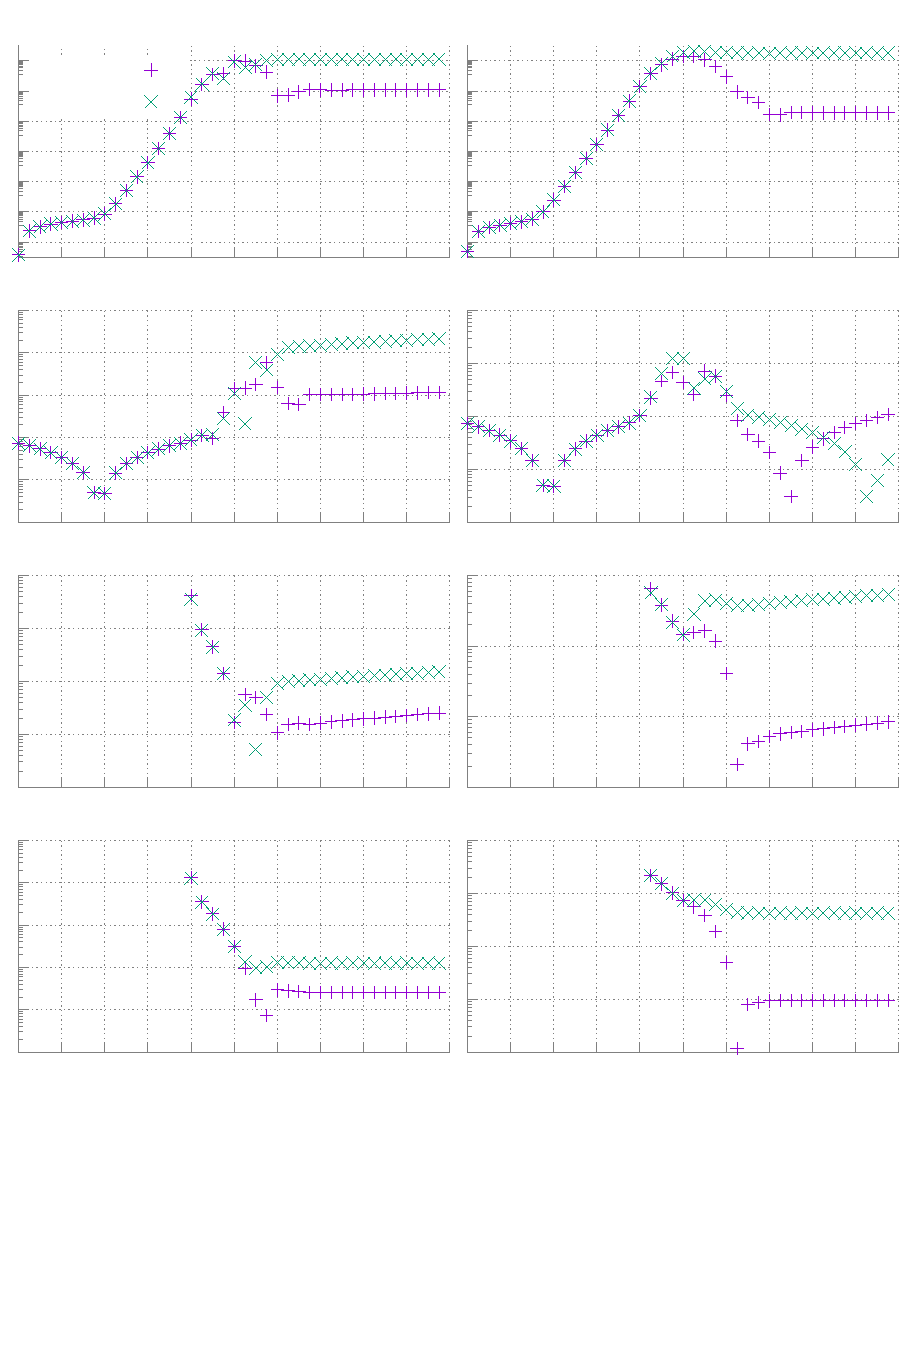
\includegraphics{/home/s1992054/NAQMD/src/SurfaceHopping/plots/sh_trajectories}}%
    \gplfronttext
  \end{picture}%
\endgroup
